% !TeX root = ../main.tex
\section{Methodology}

\subsection{Overview}
 
% 1、先介绍backbone
% 2、关注的另一块
This paper proposes a novel architecture for historical document text recognition. The overview framework is shown in Fig.\ref{fig:overall}. The architecture consists of three modules: a feature extraction module, a character length and weight prediction module, and a decoder module. The input image is first pre-processed, including padding and mirroring operations, to generate a 32x320 image. The image is then passed to the feature extraction network. The output features from the first, third, and fifth layers of the feature extraction network are input to an attention module to predict the character length and weight. The image features are then input to the decoder for prediction and decoding. For more details, please refer to vsdf\cite{vsdf}.

\subsection{Feature extraction network}

The feature extraction network consists of multiple ResNet layers. Traditional feature extraction networks have multiple output channels at each layer, with the number of channels increasing for deeper layers. This forms a hierarchical increasing structure, which we define as a triangle structure. This structure is used in the baseline method. We found that the triangle structure performs poorly on historical document text recognition tasks. Further research showed that the reason for the poor performance of the triangle structure is the imbalanced nature of the historical document text dataset, which leads to poor performance for tail classes. Inspired by MobileNet, we experimented with various structures for the feature extraction network, such as a reversed triangle structure, in which the shallow layers have more channels and the deep layers have fewer channels. We also tried a structure with more intermediate layers and fewer layers on the edges. We finally found that the best overall performance is achieved when the number of channels in the intermediate layers is increased, and the best performance for tail classes is also achieved.


\begin{figure}
    \begin{center}
    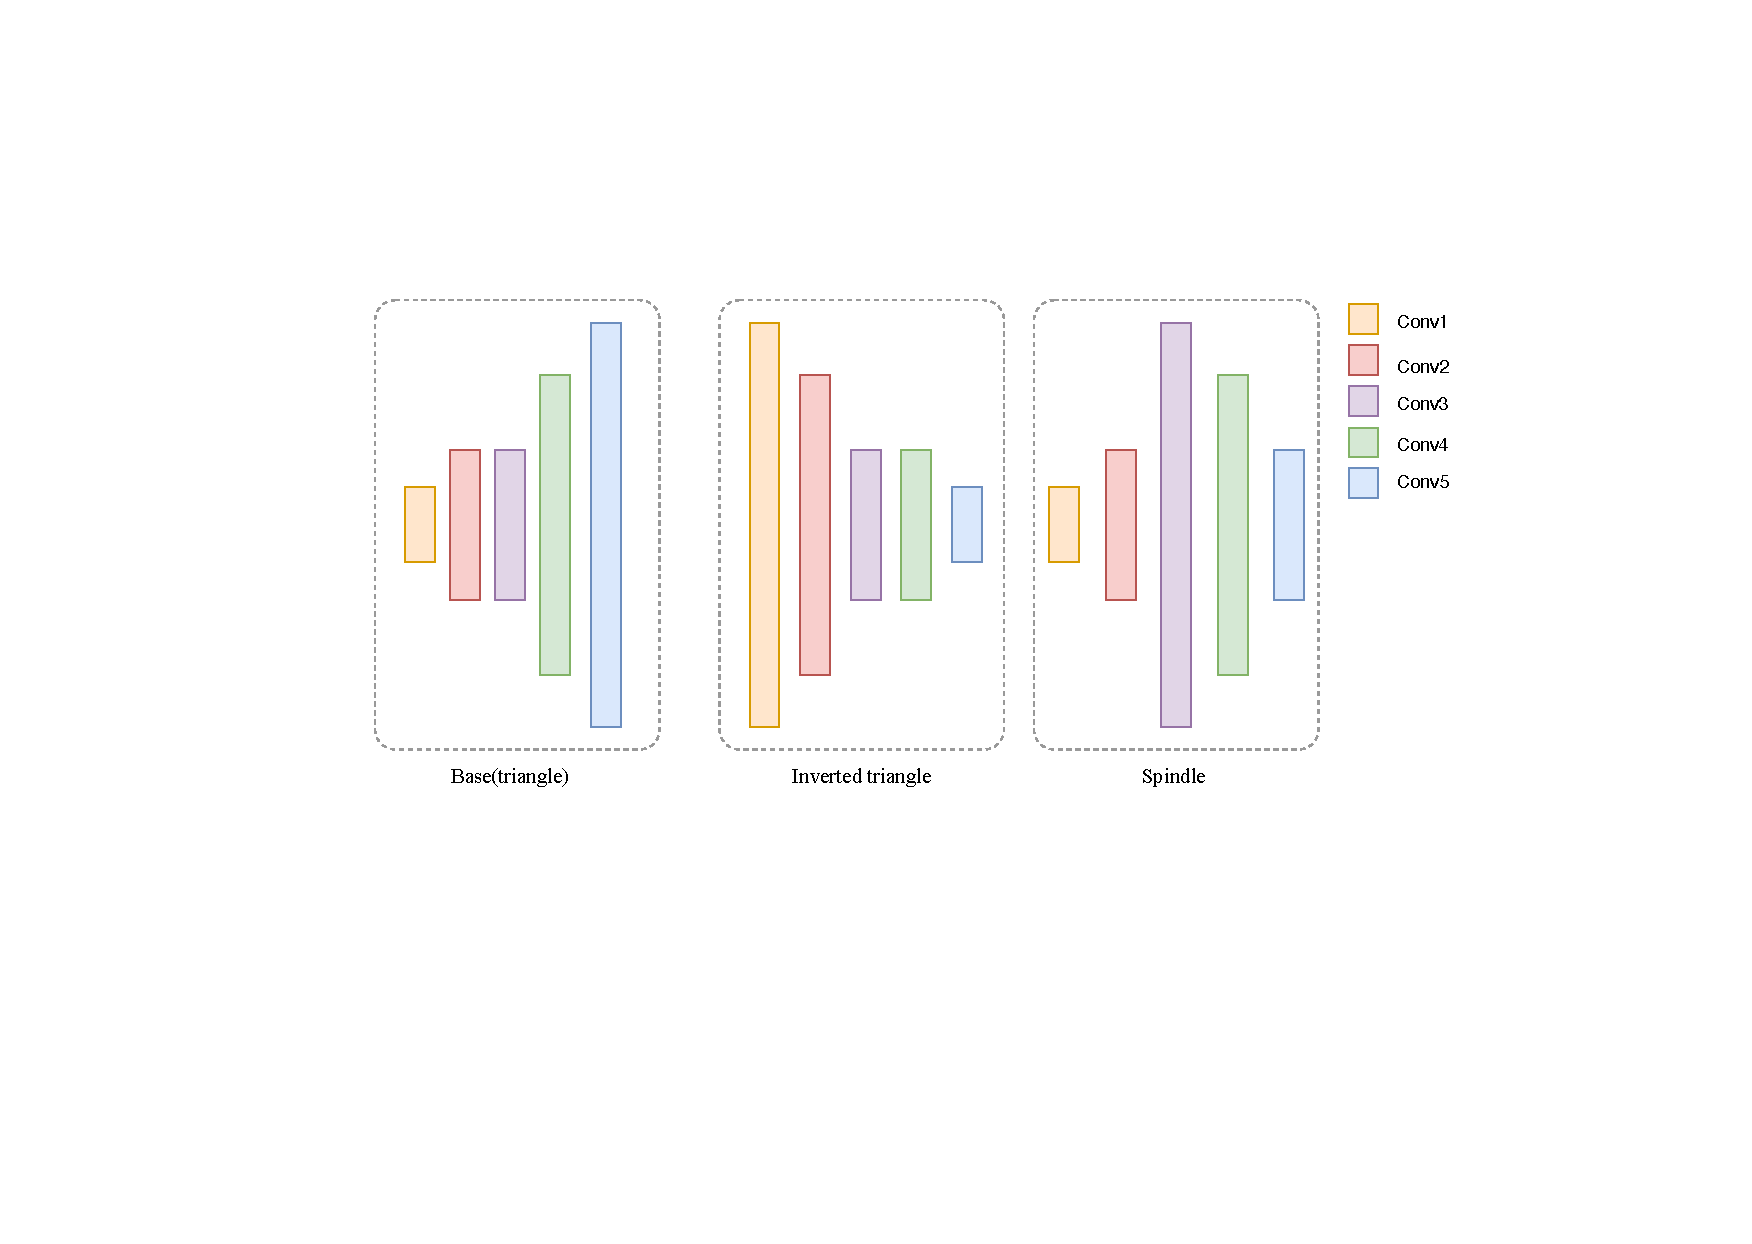
\includegraphics[width=1.0\linewidth]{figures/base_and_spindle.pdf}
    \end{center}
    \caption{The three types of feature extraction networks with different strategies are: positive triangle shape, inverted triangle shape, and spindle network shape. Different lengths represent different number of channels, for example, in the Base model, the number of channels in convolutional layers 1-5 is 32, 64, 64, 128, and 256, respectively.}
    \label{fig:base_and_spindle}
\end{figure}



\subsection{Baseline network structure and spindle-shaped network structure}
% 1、base的单loss的约束。这是关于训练的。
% 2、为什么强调参数不变,最后变成了通道数的调整参数的策略。
% 3、不同的channel,应该如何选择。


The baseline network structure is a triangle structure, with the number of channels increasing for deeper layers. The spindle-shaped network structure is a reversed triangle structure, with the number of channels decreasing for deeper layers. 
The baseline network structure consists of five ResNet layers, number of channels for each layer is as follows:[32, 64, 64, 128, 256].
The spindle-shaped network structure also consists of five ResNet layers. The number of channels for each layer is as follows: [32, 64, 256, 128, 64]. Their structures are shown in the Fig.\ref{fig:base_and_spindle} respectively.

The baseline network structure is a common choice for image classification tasks. However, we found that it performs poorly on ancient document text recognition tasks. This is because the ancient document text dataset is imbalanced, with a large number of rare characters. The baseline network structure has difficulty learning the features of rare characters, which leads to poor performance for those characters. The spindle-shaped network structure addresses this issue by increasing the number of channels in the intermediate layers. This allows the network to learn more complex features, which is beneficial for rare characters. We found that the spindle-shaped network structure achieves the best overall performance on the ancient document text recognition task, including the best performance for rare characters.

The spindle-shaped network structure is a promising architecture for ancient document text recognition. It addresses the issue of imbalanced datasets by increasing the number of channels in the intermediate layers. This allows the network to learn more complex features, which is beneficial for rare characters.
